\section{Acyclic Graphs (Trees and Forests)}
An acyclic graph has no cycles.
%
\begin{definition}{(Walk)}
Let \(G = (V;E)\) be a graph.
A walk \(w = (v_1; e_1;\allowbreak v_2; e_2; \dots;\allowbreak v_n; e_n; v_{n+1})\) in \(G\) is an alternating sequence of vertices and edges in \(V\) and \(E\) respectively so that for all \(i = 1,\dots, n: \{v_i, v_{i+1}\} = e_i\).
A walk is called closed if \(v_1 = v_{n+1}\) and open otherwise.
A walk consisting of only one vertex is called trivial.
\end{definition}

\begin{remark}
Let \(G = (V,E)\) to each walk \(w = (v_1, e_1,\allowbreak v_2, e_2,\dots,\allowbreak v_n, e_n, v_{n+1})\) we can associated a subgraph \(H = (V_0,E_0)\) with:
\begin{enumerate}
\item  \(V_0 =\{ v_1,\dots,v_{n+1}\}\)
\item  \(E_0 =\{ e_1.\dots,e_n\}\)
\end{enumerate}
We will call this the sub-graph induced by the walk \(w\).
\end{remark}

\begin{definition}{(Length)}
The length of a walk \(w\) is the number of edges contained in it.
\end{definition}
%


\begin{definition}{(Trail)}
Let \(G = (V,E)\) be a graph.
A trail in \(G\) is a walk in which no edge is repeated.
An Eulerian trail is a trail that contains exactly one copy of each edge in \(E\).
\end{definition}

\begin{definition}{(Path)}
Let \(G = (V,E)\) be a graph.
A path in \(G\) is a non-trivial walk with no vertex and no edge repeated.
A Hamiltonian path is a path that contains exactly one copy of each vertex in \(V\).
\end{definition}




\begin{example}
We illustrate a walk, cycle, Eulerian tour and a Hamiltonian path in Figure~\ref{fig:g7}.
A walk is illustrated in Figure~\ref{fig:g7a}.
Formally, this walk can be written as:
\(w = (1, \{1, 4\},\allowbreak 4, \{4, 2\},\allowbreak 2, \{2, 3\},\allowbreak 3)\).
The cycle shown in Figure~\ref{fig:g7b} can be formally written as:
\[c = (1, \{1, 4\},\allowbreak 4,\{ 4, 2\},\allowbreak 2, \{2, 3\},\allowbreak 3,\{ 3, 1\},\allowbreak 1).\]
Notice that the cycle begins and ends with the same vertex (that's what makes it a cycle).
Also, \(w\) is a sub-walk of \(c\). Note further we could easily have represented the walk as:
\[w = (3, \{3, 2\},\allowbreak 2,\{ 2, 4\},\allowbreak 4,\{4,1\},\allowbreak 1).\]
We could have shifted the ordering of the cycle in anyway (for example beginning at vertex 2).
Thus we see that in an undirected graph, a cycle or walk representation may not be unique.
In Figure~\ref{fig:g7c} we illustrate an Eulerian Trail.
This walk contains every edge in the graph with no repeats.
We note that Vertex 1 is repeated in the trail, meaning this is not a path.
We contrast this with Figure~\ref{fig:g7d} which shows a Hamiltonian path.
Here each vertex occurs exactly once in the illustrated path, but not all the edges are included.
In this graph, it is impossible to have either a Hamiltonian Cycle or an Eulerian Tour.
\end{example}
%
\begin{figure}
\centering
\begin{subfigure}{0.24\textwidth}
  \centering
  \begin{tikzpicture}[nodestyle/.style={draw,shape=circle, fill=white, blur shadow={shadow blur steps=5}}]
  % put nodes at the corners of a pentagon
  \node[regular polygon,regular polygon sides=5,minimum size=2.5cm, shape border rotate=20] (p) {};
  \foreach\x/\y in {1/1,2/4,3/3,4/5,5/2}{
    % name nodes accordingly
    \node[nodestyle] (p\y) at (p.corner \x){\y};
  }
  % draw edges
  \draw[semithick] (p1) -- (p2);
  \draw[semithick] (p1) -- (p3);
  \draw[semithick,red] (p1) -- (p4);
  \draw[semithick] (p1) -- (p5);
  \draw[semithick,red] (p2) -- (p3);
  \draw[semithick,red] (p2) -- (p4);
\end{tikzpicture}
  \caption{\label{fig:g7a}Walk}
\end{subfigure}
\begin{subfigure}{0.24\textwidth}
  \centering
  \begin{tikzpicture}[nodestyle/.style={draw,shape=circle, fill=white, blur shadow={shadow blur steps=5}}]
  % put nodes at the corners of a pentagon
  \node[regular polygon,regular polygon sides=5,minimum size=2.5cm, shape border rotate=20] (p) {};
  \foreach\x/\y in {1/1,2/4,3/3,4/5,5/2}{
    % name nodes accordingly
    \node[nodestyle] (p\y) at (p.corner \x){\y};
  }
  % draw edges
  \draw[semithick] (p1) -- (p2);
  \draw[semithick,red] (p1) -- (p3);
  \draw[semithick,red] (p1) -- (p4);
  \draw[semithick] (p1) -- (p5);
  \draw[semithick,red] (p2) -- (p3);
  \draw[semithick,red] (p2) -- (p4);
\end{tikzpicture}
  \caption{\label{fig:g7b}Cycle}
\end{subfigure}
\begin{subfigure}{0.24\textwidth}
  \centering
  \begin{tikzpicture}[
  nodestyle/.style={
    draw,
    shape=circle,
    fill=white,
    blur shadow={shadow blur steps=5}
  },
  edgename/.style={
    fill=white,
    shape=circle,
    node font=\tiny
  },
  >={Stealth[round]}
]
  % put nodes at the corners of a pentagon
  \node[regular polygon,regular polygon sides=5,minimum size=2.5cm, shape border rotate=20] (p) {};
  \foreach\x/\y in {1/1,2/4,3/3,4/5,5/2}{
    % name nodes accordingly
    \node[nodestyle] (p\y) at (p.corner \x){\y};
  }
  % draw edges
  \draw[semithick,magenta,->] (p1) -- (p2) node [edgename,midway] {2};
  \draw[semithick,orange,<-] (p1) -- (p3) node [edgename,near end] {4};
  \draw[semithick,red,->] (p1) -- (p4) node [edgename,midway] {5};
  \draw[semithick,blue,<-] (p1) -- (p5) node [edgename,very near end] {1};
  \draw[semithick,green!60!black,->] (p2) -- (p3) node [edgename,near end] {3};
  \draw[semithick,black,<-] (p2) -- (p4) node [edgename,midway] {6};
\end{tikzpicture}
  \caption{\label{fig:g7c}Eulerian Trail}
\end{subfigure}
\begin{subfigure}{0.24\textwidth}
  \centering
  \begin{tikzpicture}[
  nodestyle/.style={
    draw,
    shape=circle,
    fill=white,
    blur shadow={shadow blur steps=5}
  },
  edgename/.style={
    fill=white,
    shape=circle,
    node font=\tiny
  },
  >={Stealth[round]}
]
  % put nodes at the corners of a pentagon
  \node[regular polygon,regular polygon sides=5,minimum size=2.5cm, shape border rotate=20] (p) {};
  \foreach\x/\y in {1/1,2/4,3/3,4/5,5/2}{
    % name nodes accordingly
    \node[nodestyle] (p\y) at (p.corner \x){\y};
  }
  % draw edges
  \draw[semithick,black,dashed] (p1) -- (p2);
  \draw[semithick,black,dashed] (p1) -- (p3);
  \draw[semithick,red,->] (p1) -- (p4) node [edgename,midway] {2};
  \draw[semithick,blue,<-] (p1) -- (p5) node [edgename,very near end] {1};
  \draw[semithick,green!60!black,->] (p2) -- (p3) node [edgename,near end] {4};
  \draw[semithick,magenta,<-] (p2) -- (p4) node [edgename,midway] {3};
\end{tikzpicture}
  \caption{\label{fig:g7d}Hamiltonian Path}
\end{subfigure}
\caption{\label{fig:g7}%
A walk (a), cycle (b), Eulerian trail (c) and Hamiltonian path (d) are illustrated.
}
\end{figure}



\begin{definition}{ (Cycle)}
A closed walk of length at least 3 and with no repeated edges besides the first vertex being the same as the last is called a cycle.
A Hamiltonian cycle is a cycle in a graph containing every vertex.
\end{definition}
%
\begin{definition}{(Acyclic Graph)}
A graph that contains no cycles is called acyclic.
\end{definition}
%
\begin{definition}{(Hamiltonian / Eulerian Graph)}
A graph \(G = (V;E)\) is said to be Hamiltonian if it contains a Hamiltonian cycle and Eulerian if it contains an Eulerian tour.
\end{definition}

%
\subsection{Trees and Forests}
%
\begin{definition}{(Connectedness)}
A graph \(G\) is connected if for every pair of vertices \(v_1\) and \(v_2\) in \(V\), \(v_2\) is reachable from \(v_1\).
If \(G\) is a digraph, then \(G\) is connected if its underlying graph is connected.
A graph that is not connected is called disconnected.
\end{definition}

\begin{definition}{(Component)}
Let \(G = (V,E)\) be a graph.
A subgraph \(H\) of \(G\) is a component of \(G\) if $H$ is connected, and
 if \(K\) is a subgraph of \(G\) and \(H\) is a proper subgraph of \(K\), then \(K\) is not connected.
%
The number of components of a graph \(G\) is written \(c(G)\).
\end{definition}
%

\begin{definition}{(Vertex Cut and Cut Vertex)}
Let \(G = (V,E)\) be a graph.
A set \(V_0 \subseteq V\) is a vertex cut if the graph \(G_0\) resulting from deleting vertices \(V_0\) from \(G\) has more components than graph \(G\).
If \(V_0 = \{v\}\) is a vertex cut, then \(v\) is called a cut vertex.
\end{definition}
%
\begin{definition}{(Edge Cut and Cut-Edge)}
Let \(G = (V,E)\) be a graph.
A set \(E_0\subseteq E\) is a edge cut if the graph \(G_0\) resulting from deleting edge \(E_0\) from \(G\) has more components than graph \(G\).
If \(E_0 = \{e\}\)is an edge cut, then \(e\) is called a cut-edge.
\end{definition}
%
\begin{definition}{(Minimal Edge Cut)}
Let \(G = (V,E)\).
An edge cut \(E_0\) of \(G\) is minimal.
if when we remove any edge from \(E_0\) to form \(E_{00}\), the new set \(E_{00}\) is no longer an edge cut.
\end{definition}

\begin{figure}
\centering
\begin{subfigure}{0.49\textwidth}
  \centering
  \pgfdeclarelayer{background layer}
\pgfdeclarelayer{foreground layer}
\pgfsetlayers{background layer,main,foreground layer}
\begin{tikzpicture}[
  nodestyle/.style={%
    draw, shape=circle, fill=white,
    node font = \small,
    blur shadow={shadow blur steps=5}}
]

  \node [nodestyle] (1) at (0,0) {1};
  \node [nodestyle] (2) at ($(1) + (20:2cm)$) {2};
  \node [nodestyle] (3) at ($(1) + (-60:1.5cm)$) {3};
  \node [nodestyle] (4) at ($(3) + (1.5cm, 0)$) {4};
  \node [nodestyle,fill=red!30] (5) at ($(2) + (-30:1.5cm)$) {5};
  \node [nodestyle] (6) at ($(5) + (30:2cm)$) {6};
  \node [nodestyle] (7) at ($(6) + (-45:1.5cm)$) {7};
  \node [nodestyle] (8) at ($(5) + (-45:1.5cm)$) {8};
  \node [nodestyle] (9) at ($(8) + (-10:1cm)$) {9};

  \graph[edge quotes={auto}] {
    (1) -- {(2),(3)};
    (2) -- (4);
    (2) -- [red] (5);
    (3) -- (4);
    (4) -- [red] (5);
    (5) -- {(6),(8)};
    (6) -- {(7),(9)};
    (7) -- (9);
    (8) -- (9);
  };

  \coordinate[above=2mm] (labelpos1) at ($(2)!0.6!(5)$);
  \coordinate[below=3.7mm] (labelpos2) at ($(4)!0.6!(5)$);

  \node (label1) at (labelpos1) {$e_1$};
  \node (label2) at (labelpos2) {$e_2$};

  \coordinate (arrow_tip1) at (5.north);
  % \coordinate (arrow_tip2) at ();
  \draw[{Stealth[round]}-] (arrow_tip1) -- ++ (80:1cm) node [above] {Cut Vertex};
  % \draw[{Stealth[round]}-] (arrow_tip1) -- ++ (-80:1cm) node [below] {Articulation Point};

  \begin{pgfonlayer}{background layer}
    \draw[dashed] plot [smooth cycle] coordinates{
    (2.east)
    (4.north east)
    ($(4.south east)+(-40:0.5cm)$)
    ($(4.south east)+(10:1cm)$)
    (5.south west)
    (5.north west)
    ($(5.north)+(100:5mm)$)
    ($(2.east)+(60:5mm)$)
    };
  \end{pgfonlayer}

  \draw [{Stealth[round]}-]
  ($(4.south east)+(-20:7mm)$)
  -- ++ (-10:5mm) node [right]{Edge Cut};
\end{tikzpicture}


  \caption{\label{fig:g9a}{Edge Cut and Cut Vertex}}

\end{subfigure}
\begin{subfigure}{0.49\textwidth}
  \centering
  \pgfdeclarelayer{background layer}
\pgfdeclarelayer{foreground layer}
\pgfsetlayers{background layer,main,foreground layer}
\begin{tikzpicture}[
  nodestyle/.style={%
    draw, shape=circle, fill=white,
    node font = \small,
    blur shadow={shadow blur steps=5}}
]
  \node [nodestyle] (1) at (0,0) {1};
  \node [nodestyle,fill=red!30] (2) at ($(1) + (20:2cm)$) {2};
  \node [nodestyle] (3) at ($(1) + (-60:1.5cm)$) {3};
  \node [nodestyle,fill=red!30] (4) at ($(3) + (1.5cm, 0)$) {4};
  \node [nodestyle] (5) at ($(2) + (-30:1.5cm)$) {5};
  \node [nodestyle] (6) at ($(5) + (-10:1.5cm)$) {6};
  \node [nodestyle] (7) at ($(6) + (45:1.5cm)$) {7};
  \node [nodestyle] (8) at ($(6) + (-45:1.5cm)$) {8};
  \node [nodestyle] (9) at ($(6) + (2cm,0)$) {9};

  \graph[edges=semithick]{
    (1) -- {(2),(3)};
    (2) -- (4);
    (2) -- (5);
    (3) -- (4);
    (4) -- (5);
    (5) -- [red] (6);
    (6) -- {(7),(8),(9)};
    (7) -- (9);
    (8) -- (9);
  };

  \coordinate[above=2mm] (labelpos) at ($(5)!0.5!(6)$);
  \node (label) at (labelpos) {$e_1$};
  \draw [{Stealth[round]}-] (label) -- ++ (110:1cm) node [above] {Cut Edge};

  \begin{pgfonlayer}{background layer}
    \draw[dashed] plot [smooth cycle] coordinates {
      ($(2.north)+(90:3mm)$)
      ($(2.east)+(45:4mm)$)
      ($(4.north east)+(40:3mm)$)
      ($(4.south east)+(-45:3mm)$)
      ($(4.south west)+(-135:3mm)$)
      ($(2.west) + (180:3mm)$)
    };
  \end{pgfonlayer}

  \draw [{Stealth[round]}-]
  ($(4.south east)+(-45:3.1mm)$)
  -- ++ (-10:5mm) node [right]{Vertex Cut};

\end{tikzpicture}
  \caption{\label{fig:g9b} Vertex Cut and Cut Edge}
\end{subfigure}
\caption{\label{fig:g9}
We illustrate a vertex cut and a cut vertex (a singleton vertex cut) and an edge cut and a cut edge (a singleton edge cut).
Cuts are sets of vertices or edges whose removal from a graph creates a new graph with more components than the original graph.
}
\end{figure}
%
\begin{example}
In Figure~\ref{fig:g9}, we illustrate a vertex cut and a cut vertex (a singleton vertex cut) and an edge cut and a cut edge (a singleton edge cut).
Note that the edge-cut in Figure~\ref{fig:g9a} is minimal and cut-edges are always minimal.
A cut-edge is sometimes called a bridge because it connects two distinct components in a graph.
Bridges (and small edge cuts) are a very important part of social network analysis because they represent connections between different communities.
To see this, suppose that (for example) Figure~\ref{fig:g9b} represents the communications connections between individuals in two terrorist cells.
The fact that Member 5 and 6 communicate and that these are the only two individuals who communicate between these two cells could be important for finding a way to capture or disrupt this small terrorist network.
\end{example}
%
\begin{theorem}
Let \(G = (V,E)\) be a connected graph and let \(e \in E\).
Then \(G_0 = G-\{e\}\) is connected if and only if \(e\) lies on a cycle in \(G\).
\end{theorem}
%
\begin{proof}
Recall a graph \(G\) is connected if and only if for every pair of vertices \(v_1\) and \(v_{n+1}\) there is a walk \(w\) from \(v_1\) to  \( v_{n+1}\) with: \(w = (v_1, e_1, v_2,\dots,v_n, e_n, v_{n+1})\).
Let \(G_0 = G-\{e\}\).
Suppose that \(e\) lies on a cycle \(c\) in \(G\) and choose two vertices \(v_1\) and \(v_{n+1}\) in \(G\).
If \(e\) is not on any walk \(w\) connecting \(v_1\) to \(v_{n+1}\) in \(G\) then the removal of \(e\) does not affect the reachability of \(v_1\) and \(v_{n+1}\) in \(G_0\).
Therefore assume that \(e\) is in the walk \(w\).
The fact that \(e\) is in a cycle of \(G\) implies we have vertices \(u_1,\dots,u_m\) and edges \(f_1,\dots f_M\) so that: \(c = (u_1,f_1,\dots,u_m,f_m,u_1)\) is a cycle and \(e\) is among the \(f_1,\dots,f_m\).
Without loss of generality, assume that \(e = f_m\) and that \(e = \{u_m, u_1\}\) (If otherwise, we can re-order the cyle to make this true).
Then in \(G_0\) we will have the path: \(c_0 = (u_1, f_1,\dots,i_m)\).
The fact that \(e\) is in the walk \(w\) implies there are vertices \(v_i\) and \(v_{i+1}\) so that \(e = \{v_i, v_{i+1}\}\) (with \(v_i = u_1\) and \(v_{i+1} = u_m\)).
In deleting \(e\) from \(G\) we remove the sub-walk \((v_i, e, v_{i+1})\) from \(w\).
But we can create a new walk with structure: \(w_0 = (v_1, e_1,\dots,;\allowbreak v_i, f_1, u_2,\dots,\allowbreak u_{m-1},f_m,u_m,\dots,\allowbreak e_n,v_{n+1})\).
This is illustrated in Figure~\ref{fig:g10}.
\end{proof}
%
\begin{figure}
\centering
\begin{tikzpicture}[
  nodestyle/.style={%
    draw, shape=circle, fill=white, minimum size=0.35cm,
    blur shadow={shadow blur steps=5}}
]
\node[nodestyle] (v1) at (0,0) {};
\node[nodestyle] (v2) at ($(v1) + (1,0)$) {};
\node[nodestyle] (v3) at ($(v2) + (1.5,0)$) {};

\node[%
  regular polygon,
  regular polygon sides=7,
  minimum size=2cm,
] (p) at (4,0.91) {};

\foreach\x in {1,3,4,5,6,7}{
  % name nodes accordingly
  \node[nodestyle] (p\x) at (p.corner \x){};
};

\node[nodestyle] (v4) at ($(p5) + (1.5,0)$) {};
\node[nodestyle] (v5) at ($(v4) + (1,0)$) {};
\node[nodestyle] (v6) at ($(v5) + (1,0)$) {};

\graph[edge quotes={auto}]{
  (v1) -- (v2);
  (v2) -- [dotted, ultra thick] (v3);
  (v3) -- (p4);
  (p3) -- [red,"$u_1$" black] (p4)
       -- [ultra thick, "\large$e$"] (p5)
       -- [red, "$u_m$" black] (p6)
       -- [red] (p7)
       -- [red] (p1)
       -- [dotted, ultra thick] (p3);
  (p5) -- [dotted, ultra thick] (v4);
  (v4) -- (v5); (v5) -- (v6);
};

% Labels
\node at (v1) [below=7pt] {$v_1$};
\node at (v2) [below=7pt] {$v_2$};
\node at (p4) [below=7pt] {$v_i$};
\node at (p5) [below=7pt] {$v_{i+1}$};
\node at (v6) [below=7pt] {$v_{n+1}$};

% Arrow on top
\coordinate[above=4mm] (v1_top) at (v1);
\coordinate[above=4mm] (v3_top) at ($(v3)!0.2!(p4)$);
\coordinate (p3_near) at ($(p3.west)-(4mm,0)$);
\coordinate[above=4mm] (p1_near1) at (p1.west);
\coordinate[above=4mm] (p1_near2) at (p1.east);
\coordinate (p7_near) at ($(p7.east)+(30:3mm)$);
\coordinate (p6_near) at ($(p6.east)+(10:2.5mm)$);
\coordinate[above=4mm] (p5_top) at ($(p5)!0.6!(v4)$);
\coordinate[above=4mm] (v6_top) at (v6.east);

\draw[-{Stealth[round,length=2mm]}] (v1_top) -- (v3_top);
\draw[-{Stealth[round,length=2mm]}]
  (v3_top)
  [rounded corners]-- (p3_near)
  [rounded corners]-- (p1_near1)
  [rounded corners]-- (p1_near2)
  [rounded corners]-- (p7_near)
  [rounded corners]-- (p6_near)
  [rounded corners]-- (p5_top);
\draw[-{Stealth[round,length=2mm]}] (p5_top) -- (v6_top);

\end{tikzpicture}
\caption{\label{fig:g10}%
If \(e\) lies on a cycle, then we can repair path \(w\) by going the long way around the cycle to reach \(v_{n+1}\) from \(v_1\).
}
\end{figure}
%

%
\begin{definition}{ (Forests and Trees)}
Let \(G = (V;E)\) be an acyclic graph.
If \(G\) has more than one component, then \(G\) is called a forest.
If \(G\) has one component, then \(G\) is called a tree.
\end{definition}
%
\begin{figure}
\centering
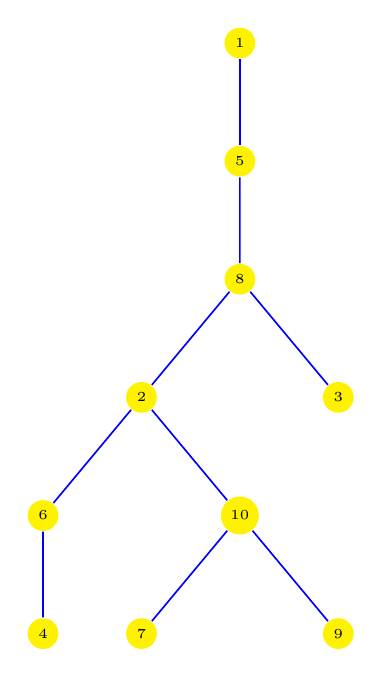
\begin{tikzpicture}[
  every node/.style={node font=\tiny, shape=circle, fill=yellow},
  level/.style={draw=blue,semithick,sibling distance=25mm}
]
  \node {1}
  child {node {5}
  child {node {8}
    child {node {2}
      child {node {6}
        child {node {4}}
      }
      child {node {10}
        child {node {7}}
        child {node {9}}
      }
    }
    child {node {3}}
  }
  };
\end{tikzpicture}
\caption{\label{fig:g8}%
A tree is shown.
Imagining the tree upside down illustrates the tree like nature of the graph structure.
}
\end{figure}
%
\begin{example}
A randomly generated tree with 10 vertices is shown in Figure~\ref{fig:g8}.
Note that a tree (if drawn upside down) can be made to look exactly like a real tree growing up from the ground.
\end{example}
%
\begin{remark}
We can define directed trees and directed forests as acyclic directed graphs.
Generally speaking, we require the underlying graphs to be acyclic rather than just having no directed cycles.
For the remainder of this section we will deal undirected trees, but results will apply to directed trees unless otherwise noted.
\end{remark}
%
\begin{definition}{ (Spanning Forest)}
Let \(G = (V,E)\) be a graph.
If \(F = (V_0;E_0)\) is an acyclic subgraph of \(G\) such that \(V = V_0\) then \(F\) is called a spanning forest of \(G\).
If \(F\) has exactly one component, then \(F\) is called a spanning tree.
\end{definition}

\begin{theorem}
If \(G = (V,E)\) is a connected graph, then there is a spanning tree \(T =(V,E_0)\) of \(G\).
\end{theorem}

\begin{proof}
We proceed by induction on the number of vertices in \(G\).
If \(|V| = 1\), then \(G\) is itself a (degenerate) tree and thus has a spanning tree.
Now, suppose that the statement is true for all graphs \(G\) with\( |V|= n\).
Consider a graph \(G\) with \(n+1\) vertices.
Choose an arbitrary vertex \(v_{n+1}\) and remove it and all edges of the form \(\{v, v_{n+1}\}\) from \(G\) to form \(G_0\) with vertex set \(V_0 =\{v_1,\dots,v_n\}\).
The graph \(G_0\) has \(n\) vertices and may have \(m\geq 1\) components (\(m > 1\) if \(v_{n+1}\) was a cut-vertex).
By the induction hypothesis, there is a spanning tree for each component of \(G_0\) since each of these components has at most \(n\) vertices.
Let \(T_1,\dots,T_m\) be the spanning trees for these components.
Let \(T_0\) be the acyclic subgraph of \(G\) consisting of all the components spanning trees.
For each spanning tree, choose exactly one edge of the form \(e(i) = \{v_{n+1}, v(i)\}\), where \(v(i)\) is a vertex in component \(i\) and add this edge to \(T_0\).
It is easy to see that no cycle is created in \(T\) through these operations because by construction, each edge \(e(i)\) is a cut-edge and by Corollary 3.43 it cannot lie on a cycle. The graph \(T\) contains every vertex of \(G\) and is connected and acyclic.
Therefore it is a spanning tree of \(G\).
The theorem then follows by induction.
\end{proof}
%
\begin{corollary}
Every graph \(G = (V,E)\) has a spanning forest \(F = (V,E_0)\).
\end{corollary}
